\documentclass[10pt, letterpaper]{article}

% Packages:
\usepackage[
    ignoreheadfoot, % set margins without considering header and footer
    top=2 cm, % seperation between body and page edge from the top
    bottom=2 cm, % seperation between body and page edge from the bottom
    left=2 cm, % seperation between body and page edge from the left
    right=2 cm, % seperation between body and page edge from the right
    footskip=1.0 cm, % seperation between body and footer
    % showframe % for debugging
]{geometry} % for adjusting page geometry
\usepackage{titlesec} % for customizing section titles
\usepackage{tabularx} % for making tables with fixed width columns
\usepackage{array} % tabularx requires this
\usepackage[dvipsnames]{xcolor} % for coloring text
\definecolor{primaryColor}{RGB}{0, 79, 144} % define primary color
\usepackage{enumitem} % for customizing lists
\usepackage{fontawesome5} % for using iconsac
\usepackage{amsmath} % for math
\usepackage{graphicx} % for the profile photo
\usepackage[
    pdftitle={VINH-KHUONG TRUONG's CV},
    pdfauthor={VINH-KHUONG TRUONG},
    pdfcreator={LaTeX with RenderCV},
    colorlinks=true,
    urlcolor=primaryColor
]{hyperref} % for links, metadata and bookmarks
\usepackage[pscoord]{eso-pic} % for floating text on the page
\usepackage{calc} % for calculating lengths
\usepackage{bookmark} % for bookmarks
\usepackage{lastpage} % for getting the total number of pages
\usepackage{changepage} % for one column entries (adjustwidth environment)
\usepackage{paracol} % for two and three column entries
\usepackage{ifthen} % for conditional statements
\usepackage{needspace} % for avoiding page brake right after the section title
\usepackage{iftex} % check if engine is pdflatex, xetex or luatex

% Ensure that generate pdf is machine readable/ATS parsable:
\ifPDFTeX
    \input{glyphtounicode}
    \pdfgentounicode=1
    % \usepackage[T1]{fontenc} % this breaks sb2nov
    \usepackage[utf8]{inputenc}
    \usepackage{lmodern}
\fi



% Some settings:
\AtBeginEnvironment{adjustwidth}{\partopsep0pt} % remove space before adjustwidth environment
\pagestyle{empty} % no header or footer
\setcounter{secnumdepth}{0} % no section numbering
\setlength{\parindent}{0pt} % no indentation
\setlength{\topskip}{0pt} % no top skip
\setlength{\columnsep}{0cm} % set column seperation
\makeatletter
\let\ps@customFooterStyle\ps@plain % Copy the plain style to customFooterStyle
\patchcmd{\ps@customFooterStyle}{\thepage}{
    \color{gray}\textit{\small VINH-KHUONG TRUONG - Page \thepage{} of \pageref*{LastPage}}
}{}{} % replace number by desired string
\makeatother
\pagestyle{customFooterStyle}

\titleformat{\section}{\needspace{4\baselineskip}\bfseries\large}{}{0pt}{}[\vspace{1pt}\titlerule]

\titlespacing{\section}{
    % left space:
    -1pt
}{
    % top space:
    0.3 cm
}{
    % bottom space:
    0.2 cm
} % section title spacing

\renewcommand\labelitemi{$\circ$} % custom bullet points
\newenvironment{highlights}{
    \begin{itemize}[
        topsep=0.10 cm,
        parsep=0.10 cm,
        partopsep=0pt,
        itemsep=0pt,
        leftmargin=0.4 cm + 10pt  % Standard left margin for highlights
    ]
}{
    \end{itemize}
} % new environment for highlights

\newenvironment{highlightsforbulletentries}{
    \begin{itemize}[
        topsep=0.10 cm,
        parsep=0.10 cm,
        partopsep=0pt,
        itemsep=0pt,
        leftmargin=10pt
    ]
}{
    \end{itemize}
} % new environment for highlights for bullet entries


\newenvironment{onecolentry}{
    \begin{adjustwidth}{
        0.2 cm + 0.00001 cm
    }{
        0.2 cm + 0.00001 cm
    }
}{
    \end{adjustwidth}
} % new environment for one column entries

\newenvironment{twocolentry}[2][]{
    \onecolentry
    \def\secondColumn{#2}
    \setcolumnwidth{\fill, 4.5 cm}
    \begin{paracol}{2}
}{
    \switchcolumn \raggedleft \secondColumn
    \end{paracol}
    \endonecolentry
} % new environment for two column entries

% HEADER ENVIRONMENT DEFINITION (Restored closer to original)
\newenvironment{header}{
    \setlength{\topsep}{0pt}\par\kern\topsep\centering\linespread{1.5} % Original linespread
}{
    \par\kern\topsep
} % new environment for the header



% save the original href command in a new command:
\let\hrefWithoutArrow\href

% new command for external links:
\renewcommand{\href}[2]{\hrefWithoutArrow{#1}{\ifthenelse{\equal{#2}{}}{ }{#2 }\raisebox{.15ex}{\footnotesize \faExternalLink*}}}



\begin{document}
\pagestyle{empty}

\newcommand{\cvname}{TRƯƠNG VĨNH KHƯƠNG}
\newcommand{\AND}{\unskip
    \cleaders\copy\ANDbox\hskip\wd\ANDbox
    \ignorespaces
}
\newsavebox\ANDbox
\sbox\ANDbox{}

% Name is provided by the including file (main.tex / main_vi.tex / cover letters)
% so the English and Vietnamese builds can share this contact block.
\providecommand{\cvname}{VINH-KHUONG TRUONG}

% Contact block, reused with and without the profile photo
\newcommand{\headercontent}{%
    \begin{header}
        \textbf{\fontsize{24 pt}{24 pt}\selectfont \cvname}
        \vspace{0.3cm}

        \normalsize
        \mbox{{\color{black}\footnotesize\faPhone*}\hspace*{0.13cm}0867084729}%
        \kern 0.25cm \AND \kern 0.25cm
        \mbox{{\color{black}\footnotesize\faEnvelope[regular]}\hspace*{0.13cm}\hrefWithoutArrow{mailto:trvinhkhuong@gmail.com}{trvinhkhuong@gmail.com}}%
        \kern 0.25cm \AND \kern 0.25cm
        \mbox{{\color{black}\footnotesize\faGithub}\hspace*{0.13cm}\hrefWithoutArrow{https://github.com/truongvinhkhuong}{github.com/truongvinhkhuong}}%
    \end{header}
}

% Drop an `image.jpg` into the repository root to show a profile photo.
% Without it the header simply renders full width.
\IfFileExists{image.jpg}{%
    \noindent
    \begin{minipage}[c]{0.78\textwidth}
        \headercontent
    \end{minipage}\hfill
    \begin{minipage}[c]{0.2\textwidth}
        \raggedleft
        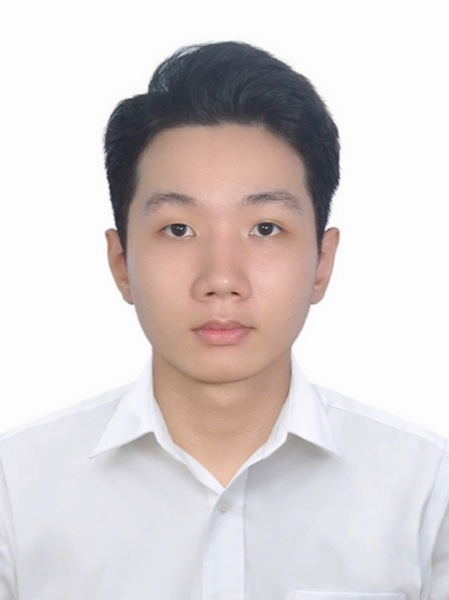
\includegraphics[width=2.5cm,height=3.5cm,keepaspectratio]{image.jpg}
    \end{minipage}
}{%
    \headercontent
}

\vspace{0.3 cm}


\vspace{0.5cm}

\begin{onecolentry}

Kính gửi Anh/Chị phụ trách tuyển dụng,

\vspace{0.2cm}

Tôi viết thư này để bày tỏ mong muốn ứng tuyển vị trí kỹ sư phần mềm tại Quý công ty. Là một Software Developer với gần hai năm kinh nghiệm phát triển sản phẩm full-stack end-to-end --- từ thiết kế hệ thống, kiến trúc API cho tới triển khai và vận hành production --- tôi tin mình có thể đóng góp thiết thực cho đội ngũ của Quý công ty.

\vspace{0.2cm}

Ở vị trí hiện tại tại \textbf{Truong Dinh Holdings}, tôi làm việc trên cả hệ thống nội bộ doanh nghiệp lẫn sản phẩm hướng khách hàng. Tôi tham gia migration theo giai đoạn từ hệ thống ERP Bravo cũ sang Odoo Community cho các mảng kho, dữ liệu khách hàng và báo cáo tài chính, đồng thời thiết kế schema cơ sở dữ liệu và RESTful API cho các module nội bộ. Tôi cũng xây dựng và triển khai \textbf{toanthang.vn} --- nền tảng doanh nghiệp song ngữ trên Next.js, NestJS, PostgreSQL và Payload CMS --- cùng \textbf{chatbot RAG} (FastAPI, LlamaIndex, Qdrant) trả lời câu hỏi khách hàng dựa trên tài liệu công ty, với pipeline BullMQ xử lý tài liệu và đánh chỉ mục ở nền.

\vspace{0.2cm}

Với vai trò \textbf{Founding Engineer tại UMIC (umic.ai)}, tôi thiết kế kiến trúc nền tảng SaaS multi-tenant về digital marketing ứng dụng AI từ con số không. Tôi xây dựng Multi-Agent AI Content Planner trên LangChain.js và LangGraph --- điều phối 5 agent chuyên biệt với luồng streaming thời gian thực qua SSE --- và thiết kế engine ``Business DNA'' chuẩn hoá bộ nhận diện thương hiệu thành ngữ cảnh sẵn sàng cho LLM, kèm prompt builder động, quản lý token và caching Redis. Song song đó tôi phát triển giao diện AI chat đa phương thức, tính năng đăng bài đa nền tảng và thư viện UI component mà toàn bộ sản phẩm vận hành trên đó.

\vspace{0.2cm}

Những vị trí trước đó đã bồi đắp nền tảng ấy: tự động hoá quy trình với n8n và Python tại \textbf{BBI}, phát triển full-stack với Python/Flask và Vue.js tại \textbf{VNGroup Tourist}, và giảng dạy lập trình tại \textbf{Trường Công nghệ MindX} --- nơi việc review code và giải thích khái niệm cho học viên giúp tôi rèn khả năng trình bày các quyết định kỹ thuật một cách rõ ràng.

\vspace{0.2cm}

\textbf{Những gì tôi mang lại:}

\vspace{0.1cm}

\begin{highlights}
    \item \textbf{Phát triển full-stack:} Node.js/NestJS, FastAPI, React/Next.js, TypeScript, PostgreSQL, Redis, Prisma
    \item \textbf{AI \& hệ thống RAG:} LangChain.js, LangGraph, LlamaIndex, Qdrant, điều phối multi-agent, giao diện đa phương thức
    \item \textbf{DevOps \& chất lượng:} Docker, Nginx, CI/CD, giám sát Prometheus/Loki, kiểm thử Jest và Cypress, SonarQube
    \item \textbf{Làm chủ sản phẩm:} Đưa tính năng từ yêu cầu tới production, bao gồm migration ERP và xây dựng SaaS từ đầu
\end{highlights}

\vspace{0.2cm}

Tôi hứng thú với những công việc mà kỹ thuật tạo ra giá trị kinh doanh thực tế --- biến các quy trình rời rạc thành hệ thống mà mọi người thực sự tin dùng. Tôi rất mong có cơ hội trao đổi thêm để làm rõ mức độ phù hợp của mình với nhu cầu của đội ngũ.

\vspace{0.4cm}

Trân trọng,\\
\textbf{Trương Vĩnh Khương}

\end{onecolentry}

\end{document}
